\documentclass{article}
\newcommand{\exptitle}{Pulsed Nuclear Magnetic Resonance}
\newcommand{\course}{PHYS3117 - Physics Labotory}

\input{../../preamble.tex}

\section{Introduction}

\section{Theory}

Atomic nuclei carry protons and neutrons, which both have a property known as spin angular momentum. Nuclei with non-zero spin possess a magnetic dipole moment, $\mu$, which is proportional to the spin angular momentum, $S$,

\begin{equation} \label{eqn:1}
    \vec{\mu} = \gamma \vec{S},
\end{equation}

where $\gamma$ is the gyromagnetic ratio, which is a constant that is unique to specific nuclei. 

\subsection{Larmor Frequency}

If we place this magnetic moment in a magnetic field, $\mathbf{B}$, it will experience a torque, $\mathbf{\tau}$ equal to $\mathbf{\mu} \times \mathbf{B}$, as the field rotates the dipole to be aligned. 
But the magnetic moment has an angular momentum $\vec S$ directed perpendicular to the field, causing the magnetic dipole to precess around the direction of the magnetic field. The magnetic moment is now at 
an angle of $\theta$ to the magnetic field, known as the angle of precession. The torque from the magnetic field will change the direction of the angular momentum of the magnetic moment so in a small time $t$ so, 

\begin{equation}
    \Delta J = \left(S \sin{\theta}\right)\left(\omega_0 \Delta t\right),
\end{equation}

where $\omega_0$ is the frequency of the precession, known as the Larmor frequency.

Note here, there is no orbital motion so $J = S$.

The rate of change of the angular momentum is then

\begin{equation}
    \frac{dJ}{dt}=\omega_0 S \sin{\theta}.
\end{equation}

This rate of change must be equal to the applied torque so, substituing in Equation \ref{eqn:1}

\begin{align} \label{eqn:larmor_frequency}
    \tau &= \mu B \sin{\theta} = \omega_0 S \sin{\theta} \\
    \omega_0 &= \frac{\mu}{J}B \nonumber \\
    &= \gamma B. \nonumber 
\end{align}

\subsection{Rotating frame of reference}
We can transform our reference frame to one that is rotating at $\omega$ about $\mathbf{B}$. We consider the magnetic 
moment as a vector in our semi-classical picture, that is,

\begin{equation}
    \vec{\mu} = \mu_x \hat{\mathbf{x}} + \mu_y \hat{\mathbf{y}} + \mu_x \hat{\mathbf{x}}.
\end{equation}

The precessing vector then would have rate of change,

\begin{align} \label{eqn:2}
    \frac{d\mu}{dt} &= \frac{\partial \mu_x}{\partial t} + \mu_x\frac{d\hat{\mathbf{x}}}{dt} + \frac{\partial \mu_y}{\partial t} + \mu_x\frac{d\hat{\mathbf{y}}}{dt} + \frac{\partial \mu_z}{\partial t} + \mu_z\frac{d\hat{\mathbf{z}}}{dt} \\
    &= \frac{\partial \mu}{\partial t} + \omega \times \mu \nonumber\\
    \frac{\partial \mu}{\partial t} &= \gamma \mu \times \left[\mathbf{B} - \frac{\omega}{\gamma}\right] \nonumber \\
    &= 0 \: \: \: \: \text{for }\omega = \omega_0 = \gamma \mathbf{B}. \nonumber 
\end{align}

We can see that if the rotating frame is rotating at the same speed as the Larmor frequency, the magnetic moment $\mu$, will appear stationary, hence resonance.

\subsection{Magnetisation}

Rather than just one magnetic moment, or one nucleus, we need to consider the whole magnetisation of the material, $M$,

\begin{equation}
    \mathbf{M}_0 = \left(\frac{\chi_0}{\mu_0}\right)\mathbf{B}.
\end{equation}

The static magnetisation $\mathbf{M}_0$ is the vector sum of all the magnetic moments from the individual nuclei. There should be a slight excess of nuclei with components of magnetic 
moments parallel to $\mathbf{B}$ rather than anti-parallel, so there should be a net magnetisation $\mathbf{M}_0$ parallel to the magnetic field. In equilibrium, there will be 
no component of magnetisation perpendicular to the magnetic field. 

If the magnetisation is perturbed, such that the magnetisation and the magnetic field are no longer aligned, the magnetisation will precess about the magnetic field, 

\begin{equation} \label{eqn:3}
    \frac{d\mathbf{M}}{dt}=\gamma \mathbf{M}\times\mathbf{B}.
\end{equation}

This precessing magnetisation can be detected if a coil was wrapped around the material. 

\subsection{Effect of Radio Frequency Pulses}

We need to first label our static magnetic field $B_0$, and place it along the z-axis, for simplicity sake, $\mathbf{B}=B_0\hat{\mathbf{z}}$. We want to now apply a plane-polarised, oscillating RF field of the form,

\begin{equation}
    \mathbf{B}_1(t) = 2B_1\cos{\omega t}\hat{\mathbf{x}}.
\end{equation}

This pulse can be decomposed into two counter-rotating components, where one component rotates opposite to the precessing magnetisation and because it is so far off resonance, can be ignored (averages out to zero). 
If the frequency of the pulse to close to resonance, that is $\omega \approx \omega_0$, the rotating field will appear static in the rotating frame. Therefore, in this rotating frame, the magnetisation only 'sees' 
the static vector $\mathbf{B}_1$. The magnetisation vector in the rotating frame will now begin to precess about $\mathbf{B_1}$ with angular frequency, $\omega_1 = \gamma B_1$, 

\begin{equation}
    \frac{\partial \mathbf{M}}{\partial t}=\gamma \mathbf{M}\times\mathbf{B}_1.
\end{equation}

If the rotating field is applied in the form of a pulse of duration $\tau_p$, then the angle of precession due to the rotating field will be 

\begin{align}
    \theta_p &= \omega_1\tau_p \\
    &= \gamma B_1 \tau_p. \nonumber 
\end{align}

We can then select $\theta_p$ to change the direction of magnetisation by applying different pulses.

\subsection{Bloch Equations}

We can see that in Equation \ref{eqn:3}, that it lacks any effects for the relaxation of the magnetisation after the perturbation. Bloch added terms to this equation based on two conditions

\begin{enumerate}
    \item Recovery of z component of magnetisation $M_z$ back to its equilibrium value $M_0$ (in absence of perturbing RF field) with time constant $T_1$, representing the longitudinal or spin-lattice relaxation time. This time 
    relates to the magnetisation exchanging energy back into the environment to achieve thermal equilibrium 
    \item Decay of the transverse components of magnetisation $M_x$ and $M_y$ over a time scale, $T_2$, characterised by the spin-spin relaxation time. Note that, in practice, the applied magnetic field $B_0$ is not homogenous so 
    spins in different parts of the material will precess at slightly different frequencies. Following a $90^\circ$ pulse, the magnetisation will de-phase, which has a time scale much shorter than $T_2$ so $T_2* < T_2$. The slightly 
    different local effective fields result in a broadening or splitting of NMR spectrum into discrete resonance peaks. The FWHM of the peak is given by $\frac{1}{\pi}T_2*$.
\end{enumerate}

The Bloch equations are derived from the differential equations, 

\begin{align}
    \frac{dM_x}{dt} &= -M_y\omega_0 - \frac{M_x}{T_2} \\
    \frac{dM_y}{dt} &= M_x\omega_0 - \frac{M_y}{T_2} \nonumber \\
    \frac{dM_z}{dt} &= \frac{\left(M_0-M_z\right)}{T_1} \nonumber 
\end{align}

which have solutions

\begin{align} \label{eqn:4}
    M_x(t) &= \left[M_x(0)\cos{\omega_0 t}+M_y(0)\sin{\omega_0 t}\right]e^{-t/T^2}\\
    M_y(t) &= \left[M_x(0)\sin{\omega_0 t}-M_y(0)\cos{\omega_0 t}\right]e^{-t/T^2}\nonumber  \\
    M_z(t) &= \left[M_z(0)-M_0\right] e^{-t/T_1} + M_0.\nonumber 
\end{align}

\section{Experimental Setup}

\subsection{Finding FID signal}
After $90^\circ$ pulse, the magnetisation will precess around $B_0$ at $\omega_0$. Initially we have 

\begin{align}
    M_z&=0 \\
    M_{\perp} &= \sqrt{M_x^2+M_y^2} = M_0
\end{align}

We know that the perpendicular magnetisation evolves with time via an exponential decay, 
\begin{equation}
    M_{\perp} = M_0 e^{-\frac{t}{T_2}}e^{-i\omega_0 t}.
\end{equation}

Now we can use Faraday's Law, 
\begin{equation}
    V(t) = -\frac{d\phi}{dt}
\end{equation}

where $\phi = \int B_{\perp}(t)\cdot dA$. We can then say that 

\begin{align} \label{eqn:induced_voltage}
    V(t) &\propto -\frac{dM_{\perp}}{dt} \\
    &\propto M_0 \left(\frac{1}{T_2^*}+i\omega_0\right)e^{-\frac{t}{T_2^*}}e^{-i\omega_0 t}. \nonumber \\
    &\propto e^{-\frac{t}{T_2^*}}e^{-i\omega_0 t} \nonumber
\end{align}

\subsection{Different samples}
In the case of solid materials and viscous liquids, with short intrinsic transverse relaxation times $T_2$, the spin-spin relaxation function can be determined directly from the FID or spectrum. However for non-viscous liquids, where 
the FID signal is affected by the magnetic field inhomogeneities, leading to a transverse relaxation time characterised by $T_2^*$.

Nuclei in diamagnetic samples will be partially screened from the full effect of the applied static magnetic field, representing a 'chemical shield'. This shield 
arises from the electron cloud of the atom, once the magnetic field is applied, it will induce a counter magnetic field, reducing the effect of the applied magnetic field.
The inhomogenuity of the sample is then reflected in the differences in precession frequencies distributed in the spins in the sample. For liquids, this screening is isotropic
(as the motion of the atoms are random). The field then experienced by a nucleus is then reduced to 

\begin{equation}
    B = B_0 (1-\sigma)
\end{equation}

where $\sigma$ is a dimensionless, chemical shielding constant. The corresponding precession frequency is then 
\begin{equation}
    \omega = \gamma(1-\sigma)B_0
\end{equation}

and the difference in average precession for two groups of nuclei (of the same atomic species but in different samples) is then

\begin{equation}
    \Delta \omega = \gamma(\sigma_2 - \sigma_1)B_0.
\end{equation}

The chemical shift, $\delta$, is then calculated as a fraction of the reference field/frequency,
\begin{equation} \label{eqn:chem_shift}
    \delta = \left(\frac{\Delta \omega}{\omega_{\text{ref}}}\right)\times10^6,
\end{equation}

given in ppm.

\subsection{Measuring the characteristic times}

To measure $T_1$, we use a pulse sequence by first perturbing the magnetisation (aligned with the z-axis), with either a $90^\circ$ or $180^\circ$ pulse, then letting the magnetisation recover over time $\tau$. After $\tau$, the magnetisation 
is 'read out' by applying a $90^\circ$ pulse and recording the FID. 

In the first case, where we first perturb with a $90^\circ$ pulse (saturation recovery), we want to equalise the populations of states, corresponding to an infinite spin temperature state. During the relaxation delay $\tau$, the transverse 
magnetisation de-phases and the longitudinal component recovers, so the FID amplitude,

\begin{equation}
    M_z(\tau)=M_0\left(1-e^{-\tau/T_1}\right).
\end{equation}

To help us obtain $T_1$, we can make an approximation, in liquid-like samples and biological materials, 

\begin{equation}
    M_y(t)=M_z e^{-t/T_2*}.
\end{equation}

In the case of starting with a $180^\circ$ pulse (inversion recovery), the sequence reverses the initial state populations and sample magnetisation, corresponding to a state of negative spin temperature. Following the $90^\circ$ pulse after 
recovery time $\tau$, the magnetisation recovers according to 
\begin{equation}
    M_z(\tau)=M_0\left(1-2e^{-\tau/T_1}\right).
\end{equation}

Here, $M_z$ will pass through zero when $\tau = T_1 \ln(2)$.

So far, we have only been able to measure $T_2^*$. In order to measure $T_2$ directly, we need to employ a 'spin echo' method. Following 
the initial $90^\circ$ pulse, we can reverse the contribution to de-phasing of the transverse magnetisation by 
applying a $180^\circ$ pulse. The spins will then rephase momentarily before starting to dephase again.

\subsection{Apparatus}

The basic layout of this experiment involves a coil wrapped around a vial of the sample material. The induced voltage on the 
coil due to the change in the magnetisation of the sample is then analysed. 

\subsubsection{Receiver Module}
The sample coil signal is first amplified by a low noise amplifier which has a fixed gain of 20 dB. This signal was subsequently 
fed into a variable gain amplifier, with a range of 0-80 dB, but we chose to set the gain to 75 dB. The goal of amplifying the 
signal, which we will discuss again with the capacitors, is to maximise signal but to a point before the signal is saturated, 
due to instrument constraints. The signal is filtered by a bandwidth filter, specifically designed for either hydrogen or 
fluorine nuclei detection. The output of the filter is sent to the inputs of the envelope detector and phase sensitive 
detectors.

\subsubsection{Synthesiser}
The objective of the synthesiser is to tune the experimental setup to the Larmor Frequency as to satisfy the condition found 
in Equation \ref{eqn:2}. One of the nice consequences of achieving resonance is that we are able to obtain the pure FID found 
in the voltage that we are measuring in Equation \ref{eqn:induced_voltage}. To do so, we need to demodulate the induced 
voltage by multiplying our synthesised continuous wave by the signal. If we consider the real component of the voltage, 

\begin{equation}
    V_{\text{real}}(t) = e^{-\frac{t}{T_2^*}}\cos(\omega_0 t),
\end{equation}

and we multiply this signal by a continous wave,

\begin{align*}
    V_{\text{sig}}(t) \cdot V_{\text{ref}}(t) &= e^{-\frac{t}{T_2^*}}\cos(\omega_0 t)\cos(\omega_{\text{ref}}t) \\
    &= \frac{1}{2}e^{-\frac{t}{T_2^*}}\left[\cos{(\omega_0 - \omega_{\text{ref}})t}+\cos{(\omega_0 + \omega_{\text{ref}})t}\right].
\end{align*}

The second term will have a very high frequency oscillation and so can be easily filtered out. If we just consider our beating term,
we can achieve resonance when this term is constant, when $\omega_{\text{ref}}=\omega_0$. We can then read the voltage from an oscilloscope
which will just return us the FID.

\subsubsection{The Permanent Magnet and LC Circuit}
The permanent magnet was used to apply the homogenous magnetic field $B_0$ along the z-axis of the sample coil. There 
were 4 shim coils to adjust the magnetic field gradient as to improve the homogeneity of the field. Optimising these 
coils were relatively easy as the coils' optimal position was when the tail of the FID curve was maximised. 

The permanent magnet was made out of NdFeB or Neodymium. This material is quite susceptible to temperature change. On the 
e-magnetsuk.com website, it cites that for a M type magnet (max working temperature of $80^\circ$C), the temperature 
coefficient is -0.12, which represents a $0.12\%$ change in the magnetic field strength for every $1^\circ$ temperature 
change. The permanent magnet is encased in a temperature cooling system, designed to keep the magnetic poles at a stable 
temperature however the manufacturer explicitly says that this system is only stable if the room temperature is kept to a 
$\pm 1^\circ$C stability.

The manual also makes an explicit note that the magnetic drift error is on the order of the difference from the Larmor frequency 
of hydrogen vs fluorine. The precession frequencies are only 6\% different and the permanent magnet will vary by several percent on different units
at ambient room temperature. The marked frequency on the magnet is merely a good place to start "tuning up" the spectrometer.

Finally, the sample inductance coil is a part of the LC circuit set up to maximise the signal obtained by the receiver module. 
The capacitor is then most importantly needed to tune the circuit to the correct driving frequency, the Larmor frequency. We 
found that our capacitor could only be tuned by rotating the screw to change the positions of the plates.

\subsection{Uncertainty Analysis}

The most challenging component of this experiment will be tuning the circuits to resonant frequency of the precessing magnetisation i.e 
finding the Larmor frequency of the sample. The desired frequency depends on the magnetic field strength which, according to the manual 
has several percentages error, on order of 6\% around the expected frequency of 21.7 MHz. 

Another large source of systematic error will 
be the position of the sample in the coil. The solenoid itself is 30 mm long with only one half it being 'reasonably' uniform. Our sample's 
vertical height was approximately 3 mm. Combined with the 'optimal' tuning of the magnetic field gradient coils, the homogeneity of the 
magnetic field is estimated to be 1\% error. The manual maintains that the magnetic field maintains homogeneity effectively, even untuned.

Furthermore, the tuning of the capacitors would contribute to bias. With some signal 
reflected back in an off-resonant circuit, this would only affect the strength of the signal received, not necessarily finding resonant 
frequency. The capacitors were tuned using a screw to change the position of the plates. We found that there were 10 full revolutions for 
the range of the capacitor so our error should be half a rotation, or 5\% error.

Lastly, the temperature of the room would drastically affect the bias in the experiment. We did have the air conditioning unit on during the whole day 
(9 am to 6 pm) however the temperature outside did change drastically that day. On September 24th, 2025, the Bureau of Meteoreolgy recorded 
an average temperature across Sydney to be 16.8$^\circ$C at 9 am and then 23.9$^\circ$C at 3 pm, with a max of 26.1$^\circ$C during midday. 
This clearly violates the stability condition stated by the manufacturer of $\pm 1 ^\circ$C, as a conservative estimate of the change of 
temperature in the room would be around that range. We can estimate the percentage on this instability error to be 1\% as the sample was 
largely confined within a temperature controlled environment inside the magnet. 

The total systematic error is then 

\begin{equation}
    \sigma_{\text{sys}} = \sqrt{0.06^2+0.01^2+0.05^2 + 0.01^2} = 0.08 = 8\%.
\end{equation}

Without any signal, the oscilloscope measured an oscillating background noise of about $\pm 10$ mV. This would encompass electronic and thermal 
noise. In terms of random flunctuation in the signal, they would be dominated by thermal motion of spins and quantum flunctuations. As there is 
a large number of spins, on scale much greater than $10^{10}$, we can assume the spin noise to be Gaussian and its standard deviation to scale with 
$\sqrt{N}$. Therefore, the percentage error would be $\frac{1}{\sqrt{N}}$, an incredibly small number so we can neglect these effects. Lastly, the 
greatest contribution to statistical error would be instrument resolution. We need to account for oscilloscope trigger, pulse length resolution, sample 
rate which would effect the sharpness of FID peaks. The largest of the resolution errors, would the pulse duration resolution. We are going up in 0.5 $\mu$s 
so the statistical error contribution would be $\pm 0.25 \: \mu$s. 

\section{Experimental Results}

We successfully obtained a value for $T_2^*$ by producing a FID seen in Figure \ref{fig:goodtime} below.

\begin{figure} [H]
    \centering
    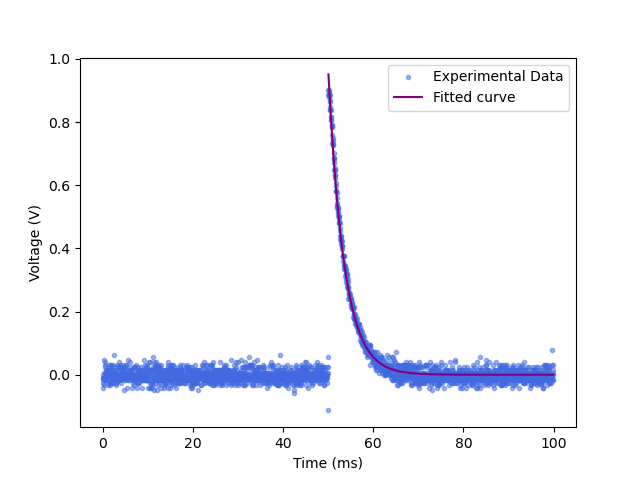
\includegraphics[width = 0.8\textwidth]{../Figures/goodtime.png}
\end{figure}

\section{Discussion}

\section{Appendix}
\subsection{Pre-lab questions}
\subsubsection{Question 1}
The Larmor angular frequency is given as 
\begin{equation}
    \omega_0 = 2\pi f_0
\end{equation}

We can substitute this into Equation \ref{eqn:larmor_frequency}, rearranging for $B_0$,

\begin{align*}
    B_0 &= \frac{\omega_0}{\gamma} \\
    &= \frac{2\pi(21.7\times10^{6})}{2.675\times10^{8}} \\
    &= 0.51 \text{ T.}
\end{align*}

\subsubsection{Question 2}
The gyromagnetic ratio of $^{19}$F nuclei is given as 
\begin{equation*}
    \gamma_{19} = 2.51815\times10^{8} \text{ s}^{-1}\text{T}^{-1}.
\end{equation*}

Therefore the Larmor Frequency, using Equation \ref{eqn:larmor_frequency} in the field in Question 1 is 

\begin{align*}
    \omega_0 &= \gamma_{19}B_0 \\
    &= 2.51815\times10^{8}\times0.5097 \\
    &=128.4\text{ MHz}
\end{align*}

or equivalently,

\begin{equation}
    f_0 = \frac{\omega_0}{2\pi} = 20.4 \text{ MHz}
\end{equation}

\subsubsection{Question 3}
The beat frequency is the difference of the two frequencies so 
\begin{equation}
    f_{\text{beat}}=21.7 - 21.696 = 0.004 \text{ MHz}.
\end{equation}

The oscillation period is simply the inverse,

\begin{equation}
    T = \frac{1}{0.004\times10^{6}}=0.00025\text{ s} = 0.25\text{ ms}
\end{equation}

\subsubsection{Question 4}
We use Equation \ref{eqn:chem_shift}, with the reference frequency being 20.0000 MHz. The chemical shift is 

\begin{align*}
    \delta &= \frac{\Delta \omega}{\omega_{\text{ref}}} \\
    &= \frac{20.0001-20.0000}{20.0000}\times10^{6} \\
    &= 5 \text{ ppm.}
\end{align*}

\end{document} 